\documentclass[10pt,twocolumn]{article}
\usepackage[utf8]{inputenc}
\usepackage[T1]{fontenc}
\usepackage{amsmath}
\usepackage{amssymb}
\usepackage{graphicx}
\usepackage{booktabs}
\usepackage{array}
\usepackage{multirow}
\usepackage{float}
\usepackage{geometry}
\usepackage{mathptmx}
\usepackage{microtype}
\usepackage{tikz}
\usepackage{url}
\usepackage{tabularx}
\usepackage[font=small,labelfont=bf]{caption}
\usetikzlibrary{arrows.meta,calc,positioning,shapes.geometric}
\geometry{margin=1in}
\setlength{\columnsep}{0.22in}
\setlength{\textfloatsep}{8pt plus 2pt minus 2pt}
\setlength{\floatsep}{6pt plus 2pt minus 2pt}
\setlength{\intextsep}{6pt plus 2pt minus 2pt}
\setlength{\dbltextfloatsep}{8pt plus 2pt minus 2pt}
\setlength{\dblfloatsep}{6pt plus 2pt minus 2pt}
\captionsetup{skip=4pt}
\setcounter{topnumber}{3}
\setcounter{dbltopnumber}{2}
\renewcommand{\topfraction}{0.9}
\renewcommand{\dbltopfraction}{0.9}
\renewcommand{\textfraction}{0.08}
\renewcommand{\floatpagefraction}{0.8}
\renewcommand{\dblfloatpagefraction}{0.8}
\flushbottom
\renewcommand{\thesection}{\Roman{section}}
\renewcommand{\thesubsection}{\Alph{subsection}}

\title{Simulation-to-Hardware Validation of Transformer-PPO for Disturbance-Resistant Retro-Propulsive Landings: Preliminary Environment Implementation and Benchmark Development}

\author{}

\date{}

\begin{document}

\maketitle

\begin{abstract}
Reusable launch vehicles require landing controllers that remain stable under nonlinear dynamics, actuator lag, and environmental disturbances. This paper presents a work-in-progress research manuscript for the project ``Simulation-to-Hardware Validation of Transformer-PPO for Disturbance-Resistant Landings,'' written from the current state of the repository rather than the full proposed end-state. The implemented code base already contains a vectorized Isaac Sim environment for an electric ducted fan (EDF) thrust-vectoring proxy vehicle, including a 6-degree-of-freedom state interface, per-fin aerodynamic force dispatch, servo lag, EDF spool dynamics, rotor reaction torque, wind drag disturbance modeling, contact/crash logic, hover and landing task definitions, and a 24-dimensional observation with a 5-dimensional action interface. In the current repository state, the environment and controller adapters are implemented, but end-to-end PID, PPO, and Gated Transformer-XL PPO (GTrXL-PPO) benchmarking has not yet been executed. Accordingly, this paper reports actual implementation status and code-level validation evidence, while also documenting provisional benchmark projections that define the intended comparative study. The repository currently passes 82 pure-Python unit tests and includes Isaac-dependent smoke tests for hover stability, vectorized RL stepping, touchdown logic, wind disturbance, and EDF spool behavior. The preliminary benchmark outlook suggests that GTrXL-PPO is likely to outperform PID and PPO in nominal and wind-disturbed landing campaigns, primarily through lower pad error, lower touchdown velocity, and improved disturbance recovery. These projected comparative values are provisional and will be replaced by empirical benchmark results as the training and evaluation campaign progresses.

\textbf{Keywords} - Reinforcement Learning, Proximal Policy Optimization, Gated Transformer-XL, Retro-Propulsive Landing, Thrust-Vectoring Control, Simulation-to-Hardware Transfer.
\end{abstract}

\section{Introduction}

Rapid booster recovery is now central to the economics of modern launch systems. Reusable first stages reduce recurring launch cost, improve operational cadence, and support future high-volume missions ranging from commercial mega-constellations to lunar logistics \cite{bushnell2018}. However, retro-propulsive landing remains a difficult control problem because the vehicle must stabilize a nonlinear, underactuated descent in the presence of uncertain disturbances, actuator dynamics, and state-estimation errors.

Classical controllers such as proportional-integral-derivative (PID) remain attractive because of their simplicity and low runtime cost, but they can lose performance when system parameters shift or disturbances become strongly nonlinear \cite{konstantopoulos2020}. Optimization-based guidance such as Sequential Convex Programming (SCP) offers strong structure and fuel-aware planning, yet trust-region limitations can cause infeasibility when the required maneuver deviates too far from the previous iterate \cite{ackmese2007}. Reinforcement learning (RL), and PPO in particular, offers a promising alternative because the policy can be trained directly against nonlinear simulation without explicit linearization \cite{schulman2017}. Still, vanilla PPO usually operates on short observation histories, which limits long-horizon reasoning during entry, descent, and landing.

Transformer-based memory addresses this limitation. Transformer-XL extends temporal context through segment recurrence \cite{dai2019}, and Gated Transformer-XL (GTrXL) improves stability for RL settings \cite{parisotto2020}. Recent aerospace work has shown strong simulated landing performance for transformer-enhanced RL under uncertainty \cite{federici2024,carradori2025}. The missing step is hardware validation: the literature still lacks a convincing simulation-to-hardware demonstration of transformer-augmented landing control on a representative physical testbed.

The research proposal for this project addresses that gap using an EDF drone with thrust-vectoring fins and a staged path from Isaac Sim, to hardware-in-the-loop (HIL), to tethered flight tests. However, the current repository has not yet completed controller training or benchmarking. This manuscript is therefore written as a work-in-progress research paper: it documents what is implemented today, explains the intended benchmark protocol, and reports clearly labeled provisional comparison values for PID, PPO, and GTrXL-PPO while empirical benchmarking is still underway.

The contributions of this work-in-progress paper are:
\begin{enumerate}
    \item We summarize the current repository implementation as a preliminary simulation artifact for EDF thrust-vectoring control, including physics, task, observation, action, and validation infrastructure.
    \item We define a benchmark protocol that is consistent with the research proposal but narrowed to the modules that exist today in code.
    \item We provide explicitly provisional benchmark tables that document the intended controller comparison while the full empirical campaign is still in progress.
\end{enumerate}

\section{Background and Related Work}

\subsection{Traditional and Learning-Based Guidance}

Powered descent guidance has historically relied on model-based methods, especially convex optimization and cascade control. Ackmese and Ploen \cite{ackmese2007} showed that convex programming can solve powered descent guidance in real time under carefully structured assumptions, but the need to remain close to a nominal trajectory creates fragility under large disturbances. PID-based methods are simpler to deploy but are sensitive to changing plant dynamics, actuator saturation, and unmodeled couplings \cite{konstantopoulos2020}.

PPO improved the practicality of RL for continuous control by stabilizing policy updates with a clipped objective \cite{schulman2017}. Hwangbo et al. \cite{hwangbo2017} further showed that learned policies can transfer from simulation to aerial hardware when the environment is randomized and the runtime policy remains computationally manageable. These results are highly relevant to EDF proxy vehicles because they suggest that an RL controller can absorb nonlinearities that are awkward to handle in hand-tuned baselines.

\subsection{Transformers for Long-Horizon Control}

Long-horizon landing problems are only partially observable when the controller sees local state snapshots but must infer slowly varying disturbances over time. Transformer-XL extends memory across segments \cite{dai2019}, while GTrXL stabilizes transformer training in RL and improves performance on tasks that require persistent memory \cite{parisotto2020}. Survey work by Li et al. \cite{li2023} argues that transformers are most useful in RL when long-range temporal credit assignment matters more than raw simplicity.

In aerospace guidance, Federici et al. \cite{federici2024} and Carradori et al. \cite{carradori2025} reported strong transformer-based landing results in simulation, including high landing success under uncertain initial conditions and disturbances. Those studies motivate the controller choice in this project, but they do not close the loop on hardware transfer.

\subsection{Research Gap}

The gap is therefore twofold. First, transformer-enhanced RL landing policies remain mostly simulation-only in the literature. Second, even within this repository, the physics environment is ahead of the controller benchmarking pipeline. The present paper sits between those two gaps: it documents an implemented environment that is ready to support future training, while honestly marking all controller comparisons as preliminary projections until the real benchmark campaign is executed.

\section{Methodology}

\subsection{Coordinate Frames and State Representation}

The environment uses two explicit coordinate conventions. The Isaac Sim world frame is right-handed and Z-up, with $+x$ forward, $+y$ left, and $+z$ up. Internal control and aerodynamic calculations use a body-fixed forward-right-down (FRD) frame with $+x$ forward, $+y$ right, and $+z$ down. The code enforces a single conversion boundary between these frames through
\begin{equation}
\mathbf{R}_{I\leftarrow F} =
\begin{bmatrix}
1 & 0 & 0 \\
0 & -1 & 0 \\
0 & 0 & -1
\end{bmatrix},
\label{eq:frd_isaac_map}
\end{equation}
where superscript $F$ denotes body-FRD coordinates and superscript $I$ denotes Isaac-aligned body coordinates. Thus,
\begin{equation}
\mathbf{v}^{I} = \mathbf{R}_{I\leftarrow F}\mathbf{v}^{F},
\qquad
\mathbf{v}^{F} = \mathbf{R}_{I\leftarrow F}^{T}\mathbf{v}^{I}.
\label{eq:frd_bidirectional}
\end{equation}

Vehicle orientation is stored as a quaternion in Isaac Lab's $(w,x,y,z)$ convention:
\begin{equation}
\mathbf{q} = [w,x,y,z]^{T}.
\end{equation}
For a local vector $\mathbf{v}$, world rotation follows the quaternion sandwich product
\begin{equation}
\mathbf{v}' = \mathbf{q}\,[0,\mathbf{v}]\,\mathbf{q}^{-1},
\label{eq:quat_rotation}
\end{equation}
which is implemented in code through the equivalent vector form. If $\mathbf{R}(\mathbf{q})$ is the rotation matrix induced by $\mathbf{q}$, then a body-FRD vector is mapped to world coordinates by
\begin{equation}
\mathbf{v}^{W} = \mathbf{R}(\mathbf{q})\,\mathbf{R}_{I\leftarrow F}\,\mathbf{v}^{F},
\label{eq:body_to_world}
\end{equation}
and a world-frame vector is mapped back to body-FRD by
\begin{equation}
\mathbf{v}^{F} = \mathbf{R}_{I\leftarrow F}^{T}\mathbf{R}(\mathbf{q})^{T}\mathbf{v}^{W}.
\label{eq:world_to_body}
\end{equation}

The per-step simulated vehicle state can therefore be summarized as
\begin{equation}
\mathbf{x}_{t} =
\left[
\mathbf{p}_{t}^{W},
\mathbf{q}_{t},
\mathbf{v}_{t}^{W},
\boldsymbol{\omega}_{t}^{W},
\boldsymbol{\delta}_{t},
\dot{\boldsymbol{\delta}}_{t},
\Omega_{t},
c_{t}
\right],
\label{eq:state_vector}
\end{equation}
where $\mathbf{p}^{W}$ is position, $\mathbf{v}^{W}$ is linear velocity, $\boldsymbol{\omega}^{W}$ is angular velocity, $\boldsymbol{\delta}\in\mathbb{R}^{4}$ are fin angles, $\dot{\boldsymbol{\delta}}\in\mathbb{R}^{4}$ are fin rates, $\Omega$ is rotor speed, and $c_t$ is the contact-state variable.

The policy acts through a 5-dimensional action vector,
\begin{equation}
\mathbf{a}_{t} =
\left[
\delta_{1}^{cmd},
\delta_{2}^{cmd},
\delta_{3}^{cmd},
\delta_{4}^{cmd},
u_{t}
\right]^{T},
\label{eq:action_vector}
\end{equation}
where $\delta_{i}^{cmd}\in[-\delta_{\max},\delta_{\max}]$ and $u_t\in[0,1]$ is normalized throttle. In the present repository, $\delta_{\max}=0.262$ rad.

\subsection{Servo and EDF Propulsion Models}

Each fin servo is modeled as a first-order actuator with rate limiting and a deadband. Let $\delta_i$ denote the actual fin angle and $\delta_i^{cmd}$ the commanded angle after clipping. The implemented dynamics are
\begin{equation}
\dot{\delta}_{i} =
\mathrm{sat}_{\dot{\delta}_{\max}}
\left(
\frac{\delta_{i}^{cmd} - \delta_i}{\tau_s}
\right),
\label{eq:servo_rate}
\end{equation}
\begin{equation}
\delta_{i,t+\Delta t} =
\mathrm{clip}\left(
\delta_{i,t} + \dot{\delta}_{i}\Delta t,
-\delta_{\max},\delta_{\max}
\right).
\label{eq:servo_integrator}
\end{equation}
After integration, a small deadband is enforced by setting $\delta_i=0$ whenever $|\delta_i|<\delta_{db}$. The current parameterization uses $\tau_s \approx 0.05$ s, $\dot{\delta}_{\max}\approx 7.54$ rad/s, and $\delta_{db}\approx 0.017$ rad.

The EDF motor is modeled with first-order spool dynamics,
\begin{equation}
\Omega_{target} = u_t \Omega_{\max},
\label{eq:omega_target}
\end{equation}
\begin{equation}
\dot{\Omega} = \frac{\Omega_{target} - \Omega}{\tau_m},
\label{eq:omega_dynamics}
\end{equation}
with optional slew-rate limiting available in the code path but not yet calibrated in the current configuration. The thrust magnitude is quadratic in rotor speed:
\begin{equation}
T = k_T \Omega^2.
\label{eq:thrust_eq}
\end{equation}

The repository defines the rotor spin/exhaust axis as
\begin{equation}
\mathbf{s}^{F} = [0,0,1]^{T},
\end{equation}
which points along $+z_F$ (downward exhaust in FRD). The body thrust applied to the airframe is therefore opposite the exhaust direction:
\begin{equation}
\mathbf{F}^{F}_{edf} = -T \mathbf{s}^{F}.
\label{eq:body_thrust}
\end{equation}

The propulsion model also computes three torque components:
\begin{equation}
\boldsymbol{\tau}_{static} = -k_Q \Omega^2 \mathbf{s}^{F},
\label{eq:static_torque}
\end{equation}
\begin{equation}
\boldsymbol{\tau}_{spool} = I_r \dot{\Omega}\,\mathbf{s}^{F},
\label{eq:spool_torque}
\end{equation}
\begin{equation}
\boldsymbol{\tau}_{gyro} = \boldsymbol{\omega}^{F}\times\left(I_r \Omega \mathbf{s}^{F}\right),
\label{eq:gyro_torque}
\end{equation}
where $I_r$ is rotor inertia and $\boldsymbol{\omega}^{F}$ is body angular velocity expressed in FRD coordinates. These terms are individually available for testing and logging.

\subsection{Fin Aerodynamics and Force Dispatch}

The four thrust-vectoring fins are modeled with a semi-empirical jet-vane formulation in the EDF exhaust stream. Let $u_t$ denote throttle and $v_{exh}$ the nominal exhaust speed. The code scales jet dynamic pressure by throttle squared:
\begin{equation}
\bar{q}_{j} = \frac{1}{2}\rho v_{exh}^{2} u_t^2.
\label{eq:jet_pressure}
\end{equation}
For fin area $S$, the normal-force and tangential-force coefficients are
\begin{equation}
C_N(\alpha) = C_{N\alpha}\alpha(1-k_{sat}\alpha^2),
\label{eq:cn}
\end{equation}
\begin{equation}
C_D(\alpha) = C_{D,0} + C_{D,\alpha^2}\alpha^2.
\label{eq:cd}
\end{equation}
The corresponding force magnitudes are
\begin{equation}
F_n = \bar{q}_{j} S C_N(\alpha),
\qquad
F_t = \bar{q}_{j} S C_D(\alpha).
\label{eq:fin_forces}
\end{equation}

In the current implementation, the normal component is the one converted into the runtime fin-local force vector used for force application, while the tangential component and a derived thrust-loss estimate are tracked diagnostically. This distinction matters because it reflects the current code state rather than a fully completed plume-interaction model.

If $\mathbf{h}_i$ is the hinge axis of fin $i$ and $\delta_i$ its actual servo angle, then the fin-local-to-body rotation is constructed through an axis-angle quaternion
\begin{equation}
\mathbf{q}_{i}^{fin} = \mathrm{AxisAngle}(\mathbf{h}_i,\delta_i),
\label{eq:axis_angle_fin}
\end{equation}
and the body-frame fin force is
\begin{equation}
\mathbf{F}_{i}^{F} = \mathbf{R}(\mathbf{q}_{i}^{fin})\,\mathbf{F}_{i}^{local}.
\label{eq:body_fin_force}
\end{equation}
The center-of-pressure offset $\mathbf{r}_i^{F}$ for each fin is loaded from asset metadata. In the optional collapsed-wrench mode, the total fin-generated moment is
\begin{equation}
\boldsymbol{\tau}^{F}_{fin} = \sum_{i=1}^{4}\mathbf{r}_i^{F}\times \mathbf{F}_{i}^{F}.
\label{eq:collapsed_torque}
\end{equation}

The default runtime mode is instead \emph{per-link force application}. Each $\mathbf{F}_{i}^{F}$ is transformed to world coordinates through (\ref{eq:body_to_world}) and applied at the transformed center-of-pressure location
\begin{equation}
\mathbf{r}_{i}^{W} = \mathbf{R}(\mathbf{q})\,\mathbf{R}_{I\leftarrow F}\,\mathbf{r}_i^{F},
\label{eq:cop_world}
\end{equation}
which allows the articulation physics to generate the resulting vehicle torque from geometry rather than from a manually synthesized body moment.

\subsection{Wind Disturbance, Observation, Reward, and Termination}

The currently implemented disturbance model includes steady wind, gusts, and body drag. With world-frame wind $\mathbf{v}^{W}_{wind}$ and world-frame vehicle velocity $\mathbf{v}^{W}$, the relative airflow is
\begin{equation}
\mathbf{v}^{W}_{rel} = \mathbf{v}^{W} - \mathbf{v}^{W}_{wind}.
\label{eq:vrel}
\end{equation}
The drag force in world coordinates is
\begin{equation}
\mathbf{F}^{W}_{drag} =
-\frac{1}{2}\rho C_{D,b}A_b \lVert \mathbf{v}^{W}_{rel}\rVert^2
\frac{\mathbf{v}^{W}_{rel}}{\lVert \mathbf{v}^{W}_{rel}\rVert},
\label{eq:drag_world}
\end{equation}
where $C_{D,b}$ and $A_b$ are the body drag coefficient and reference area. This force is transformed back to FRD coordinates using (\ref{eq:world_to_body}) before being added to the body-level wrench.

The policy observation used by the current environment is a 24-dimensional vector,
\begin{equation}
\mathbf{o}_t = \left[
\mathbf{e}_{p},
\mathbf{q},
\mathbf{v}^{F},
\boldsymbol{\omega}^{F},
h,
\boldsymbol{\delta},
\dot{\boldsymbol{\delta}},
\Omega/\Omega_{\max},
c_t
\right],
\label{eq:obs}
\end{equation}
where $\mathbf{e}_{p}=\mathbf{p}^{*}-\mathbf{p}$ is position error and $h$ is altitude above ground.

Rewards are assembled from a task-specific registry as a weighted sum
\begin{equation}
r_t = \sum_{k} w_k \phi_k(\mathbf{x}_t),
\label{eq:reward_sum}
\end{equation}
where the active terms and their weights are selected from the reward YAML associated with the task. To keep the equations readable in two-column format, the implemented rewards are written below in grouped form using the shorthand
\begin{equation}
\begin{aligned}
e_p &= \left\|\mathbf{p}-\mathbf{p}^{*}\right\|_2, \qquad
e_\theta = \sqrt{\phi^2+\theta^2}, \qquad
e_\omega = \left\|\boldsymbol{\omega}^{F}\right\|_2,\\
u_\delta &= \overline{|\boldsymbol{\delta}|}, \qquad
u_{\dot\delta} = \overline{|\dot{\boldsymbol{\delta}}|}, \qquad
v_{xy} = \left\|\mathbf{v}_{xy}^{F}\right\|_2,
\end{aligned}
\label{eq:reward_shorthand}
\end{equation}
and, for landing,
\begin{equation}
\begin{aligned}
s_{soft} &= \exp\!\left(-\max(v_z^{F},0)\right),\\
a_{pad} &= \exp\!\left(-2\left\|\mathbf{p}_{xy}-\mathbf{p}^{*}_{xy}\right\|_2\right).
\end{aligned}
\label{eq:landing_reward_shorthand}
\end{equation}

For the current hover configuration, the reward is decomposed into a stay-alive term $r_{stay}^{hover}$, a tracking term $r_{track}^{hover}$, an actuator-regularization term $r_{act}^{hover}$, and a hover-task term $r_{task}^{hover}$:
\begin{subequations}\label{eq:hover_reward_impl}
\begin{align}
r_t^{hover}
&= r_{stay}^{hover} + r_{track}^{hover}
 + r_{act}^{hover} + r_{task}^{hover}, \\
r_{stay}^{hover}
&= 1.0, \\
r_{track}^{hover}
&= -2.0\,e_p - 1.0\,e_\theta - 0.5\,e_\omega - 1.5\,v_{xy}, \\
r_{act}^{hover}
&= -0.1\,u_\delta - 0.05\,u_{\dot\delta}, \\
r_{task}^{hover}
&= 2.0\,\mathbb{1}_{hover} - 10.0\,\mathbb{1}_{contact}.
\end{align}
\end{subequations}
Here, $\mathbb{1}_{hover}=1$ when both the position error and tilt remain inside the configured success envelope, and $\mathbb{1}_{contact}=1$ when the contact state is anything other than airborne. The rationale is to combine dense tracking terms with mild actuator regularization and a strong penalty on ground contact, so the hover controller is driven toward a quiet, centered, non-touching equilibrium rather than aggressive limit cycling.

For the current landing configuration, the reward is decomposed into a stay-alive term $r_{stay}^{land}$, a tracking term $r_{track}^{land}$, a terminal-outcome term $r_{term}^{land}$, and a descent-shaping term $r_{shape}^{land}$:
\begin{subequations}\label{eq:landing_reward_impl}
\begin{align}
r_t^{land}
&= r_{stay}^{land} + r_{track}^{land}
 + r_{term}^{land} + r_{shape}^{land}, \\
r_{stay}^{land}
&= 0.5, \\
r_{track}^{land}
&= -1.0\,e_p - 1.5\,e_\theta - 0.5\,e_\omega - 0.1\,u_\delta, \\
r_{term}^{land}
&= -100.0\,\mathbb{1}_{crash} + 50.0\,\mathbb{1}_{landed} \nonumber\\
&\quad + 10.0\,a_{pad}\,\mathbb{1}_{landed}, \\
r_{shape}^{land}
&= 5.0\,s_{soft} - 2.0\,|v_z^{F} - 0.5|.
\end{align}
\end{subequations}
Here, $v_z^{F}$ is the FRD vertical velocity component, which is positive for downward motion, $\mathbb{1}_{crash}=1$ in the crashed contact state, and $\mathbb{1}_{landed}=1$ in the landed contact state. The terminal block encodes the main task objective, the shaping block improves approach behavior before touchdown, and the tracking block suppresses large pose and rate errors during the descent. This grouped form is algebraically equivalent to the implemented weighted-sum reward, but is easier to read in manuscript form.

Episode termination is triggered when any configured condition is met:
\begin{equation}
d_t =
\mathbb{1}_{crash}
\vee
\mathbb{1}_{\|\boldsymbol{\theta}\| > \theta_{max}}
\vee
\mathbb{1}_{\|\mathbf{p}-\mathbf{p}^{*}\| > e_{max}}
\vee
\mathbb{1}_{t \geq t_{max}},
\label{eq:termination}
\end{equation}
where $\boldsymbol{\theta}=[\phi,\theta]$ represents roll and pitch, $e_{max}$ is the configured altitude-error limit, and $t_{max}$ is the episode timeout derived from the task duration and the RL step period.

\subsection{Isaac Lab Environment Architecture Pattern and Force/Wrench Application}

Beyond the physical equations, the repository follows a specific Isaac Lab software pattern that is important for reproducibility. The environment is organized as a four-stage stack. First, \texttt{BaseEnvConfig} merges task, environment, disturbance, and override dictionaries through the task registry. Second, \texttt{SceneConfig} and \texttt{build\_scene()} instantiate the Isaac Lab \texttt{SimulationContext}, construct an \texttt{InteractiveScene}, clone the configured number of environments, and attach the validated vehicle articulation. Third, \texttt{TVCEnvBase.\_initialize\_physics\_systems()} wires together the articulation map, body-state interface, link-force interface, servo model, EDF model, aerodynamic model, wrench dispatcher, reset manager, and contact logic. Fourth, \texttt{TVCDirectRLEnv.step()} executes the decimated RL interaction loop.

The merged runtime configuration can be written abstractly as
\begin{equation}
\mathcal{C}
=
\mathrm{Merge}\!\left(
\mathcal{C}_{task},
\mathcal{C}_{env},
\mathcal{C}_{dist},
\mathcal{C}_{override}
\right),
\label{eq:config_merge}
\end{equation}
where $\mathcal{C}_{task}$ is the task YAML, $\mathcal{C}_{env}$ is the environment YAML, $\mathcal{C}_{dist}$ is the disturbance YAML, and $\mathcal{C}_{override}$ denotes command-line or script-level overrides. The resulting scene/runtime stack is then
\begin{equation}
\mathcal{E}
=
\mathrm{InitSystems}\!\left(
\mathrm{BuildScene}(\mathcal{C}),
\mathcal{M}_{asset},
\mathcal{P}_{vehicle},
\mathcal{P}_{edf},
\mathcal{P}_{servo}
\right),
\label{eq:env_stack}
\end{equation}
where $\mathcal{M}_{asset}$ denotes USD metadata and $\mathcal{P}_{vehicle}$, $\mathcal{P}_{edf}$, and $\mathcal{P}_{servo}$ are the parameter sets loaded from the repository YAML files.

At the RL level, one environment step is
\begin{equation}
\left(
\mathbf{o}_{t+1},
r_t,
\mathbb{1}_{term},
\mathbb{1}_{trunc}
\right)
=
\mathrm{Step}_{\mathcal{E}}(\mathbf{a}_t),
\label{eq:isaac_step}
\end{equation}
where $\mathbf{o}_{t+1}$ is the next observation, $r_t$ is the scalar reward, $\mathbb{1}_{term}$ is the termination indicator, and $\mathbb{1}_{trunc}$ is the timeout indicator. Because the environment uses decimation, each RL action is held constant over $d$ physics substeps:
\begin{equation}
\mathbf{u}_t = \mathrm{clip}(\mathbf{a}_t),
\qquad
\mathbf{x}^{(j+1)} = \Phi\!\left(\mathbf{x}^{(j)},\mathbf{u}_t,\Delta t\right),
\quad j=1,\ldots,d,
\label{eq:decimated_rollout}
\end{equation}
where $\mathbf{u}_t$ is the clamped control vector, $d$ is the decimation factor, $\Delta t$ is the physics step, and $\Phi(\cdot)$ denotes one force-application and simulation-update cycle.

In the current implementation, one substep of $\Phi(\cdot)$ consists of
\begin{equation}
\left(\boldsymbol{\delta}^{(j+1)},\Omega^{(j+1)}\right)
=
f_{act}\!\left(
\boldsymbol{\delta}^{(j)},
\Omega^{(j)},
\mathbf{u}_t,
\Delta t
\right),
\label{eq:substep_actuation}
\end{equation}
\begin{equation}
\left(\{\mathbf{F}_{i}^{F,(j+1)}\}_{i=1}^{4},\{\mathbf{r}_{i}^{F}\}_{i=1}^{4}\right)
=
f_{fin}\!\left(
\boldsymbol{\delta}^{(j+1)},
u_{thr,t}
\right),
\label{eq:substep_finforces}
\end{equation}
\begin{equation}
\mathbf{F}_{body}^{F,(j+1)}
=
\mathbf{F}_{EDF}^{F,(j+1)}
+
\mathbf{F}_{wind}^{F,(j+1)},
\label{eq:body_force_combined}
\end{equation}
\begin{equation}
\mathcal{W}^{(j+1)}
=
\mathrm{Dispatch}\!\left(
\{\mathbf{F}_{i}^{F,(j+1)}\},
\{\mathbf{r}_{i}^{F}\},
\mathbf{F}_{body}^{F,(j+1)},
\mathbf{q}^{(j+1)}
\right),
\label{eq:wrench_dispatch_step}
\end{equation}
where $f_{act}(\cdot)$ is the combined servo and EDF update, $\boldsymbol{\delta}^{(j)}$ is the fin-angle state at substep $j$, $\Omega^{(j)}$ is the rotor speed state, $u_{thr,t}$ is the held throttle command, $\mathbf{F}_{i}^{F,(j+1)}$ is the body-FRD force generated by fin $i$, $\mathbf{r}_{i}^{F}$ is the corresponding center-of-pressure offset, $\mathbf{F}_{EDF}^{F,(j+1)}$ is the EDF thrust contribution, $\mathbf{F}_{wind}^{F,(j+1)}$ is the wind/body-drag contribution, $\mathbf{q}^{(j+1)}$ is the root quaternion, and $\mathcal{W}^{(j+1)}$ denotes the external-force data written to PhysX for that substep.

The force/wrench application step supports two dispatch modes. In the default \emph{per-link force} mode, each fin force is rotated to world coordinates and applied at its world-frame center of pressure using Isaac Lab's permanent wrench composer, while EDF thrust and wind drag are applied as body-link forces. In the optional \emph{collapsed body wrench} mode, the implementation instead forms a net body force and the geometric torque in (\ref{eq:collapsed_torque}) before applying a single body wrench. Figure \ref{fig:isaac_arch_pattern} summarizes both the environment architecture pattern and the force/wrench application path.

\begin{figure*}[!t]
\centering
\begin{minipage}[t]{0.48\textwidth}
\centering
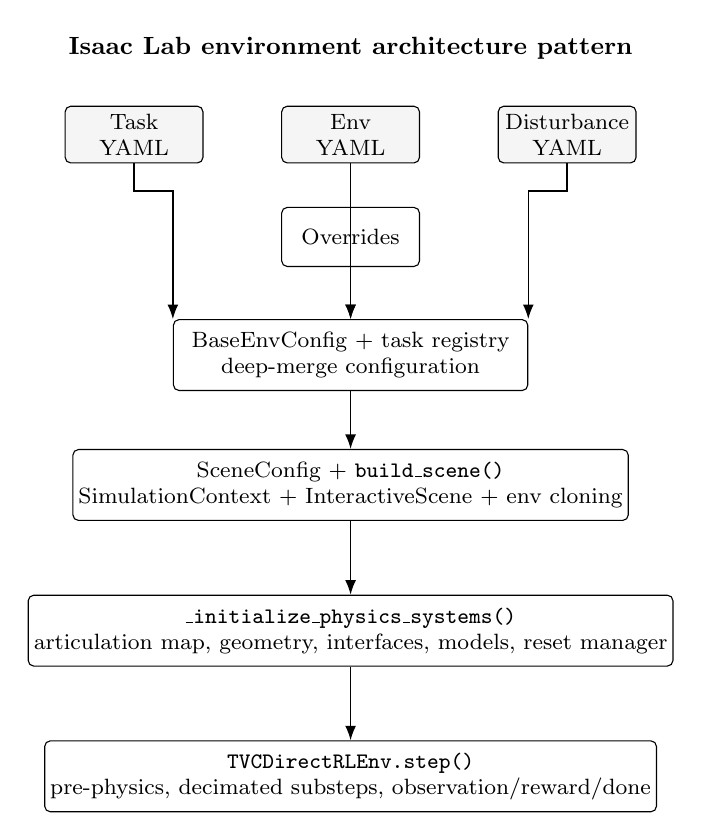
\begin{tikzpicture}[
    x=1cm,
    y=1cm,
    >={Latex[length=2mm]},
    box/.style={draw, rounded corners=2pt, align=center, minimum width=4.5cm, minimum height=0.9cm, inner sep=2pt, font=\footnotesize},
    smallbox/.style={draw, rounded corners=2pt, align=center, minimum width=1.75cm, minimum height=0.75cm, inner sep=2pt, font=\footnotesize},
    io/.style={draw, rounded corners=2pt, align=center, minimum width=1.75cm, minimum height=0.72cm, inner sep=2pt, fill=gray!8, font=\footnotesize},
    dot/.style={circle, fill, inner sep=0.8pt},
    line/.style={-Latex, line width=0.5pt}
]
\node[font=\small\bfseries] at (0,1.1) {Isaac Lab environment architecture pattern};
\node[io] (task) at (-2.75,0) {Task\\YAML};
\node[io] (env) at (0,0) {Env\\YAML};
\node[io] (dist) at (2.75,0) {Disturbance\\YAML};
\node[smallbox] (override) at (0,-1.3) {Overrides};
\node[box] (merge) at (0,-2.8) {BaseEnvConfig + task registry\\deep-merge configuration};
\node[box] (scene) at (0,-4.45) {SceneConfig + \texttt{build\_scene()}\\SimulationContext + InteractiveScene + env cloning};
\node[box] (init) at (0,-6.3) {\texttt{\_initialize\_physics\_systems()}\\articulation map, geometry, interfaces, models, reset manager};
\node[box] (step) at (0,-8.15) {\texttt{TVCDirectRLEnv.step()}\\pre-physics, decimated substeps, observation/reward/done};

\draw[line] (task.south) -- ++(0,-0.35) -| (merge.north west);
\draw[line] (env.south) -- ++(0,-0.35) -- (merge.north);
\draw[line] (dist.south) -- ++(0,-0.35) -| (merge.north east);
\draw[line] (override.south) -- (merge.north);
\draw[line] (merge) -- (scene);
\draw[line] (scene) -- (init);
\draw[line] (init) -- (step);
\end{tikzpicture}
\end{minipage}\hfill
\begin{minipage}[t]{0.48\textwidth}
\centering
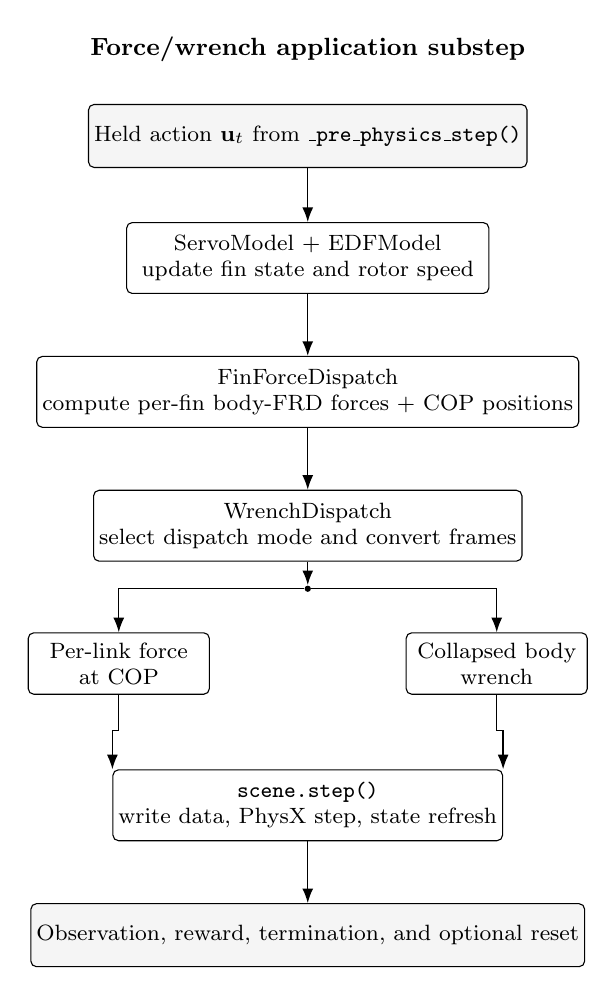
\begin{tikzpicture}[
    x=1cm,
    y=1cm,
    >={Latex[length=2mm]},
    box/.style={draw, rounded corners=2pt, align=center, minimum width=4.6cm, minimum height=0.9cm, inner sep=2pt, font=\footnotesize},
    smallbox/.style={draw, rounded corners=2pt, align=center, minimum width=2.3cm, minimum height=0.78cm, inner sep=2pt, font=\footnotesize},
    io/.style={draw, rounded corners=2pt, align=center, minimum width=4.6cm, minimum height=0.8cm, inner sep=2pt, fill=gray!8, font=\footnotesize},
    dot/.style={circle, fill, inner sep=0.8pt},
    line/.style={-Latex, line width=0.5pt}
]
\node[font=\small\bfseries] at (0,1.1) {Force/wrench application substep};
\node[io] (action) at (0,0) {Held action $\mathbf{u}_t$ from \texttt{\_pre\_physics\_step()}};
\node[box] (act) at (0,-1.55) {ServoModel + EDFModel\\update fin state and rotor speed};
\node[box] (fin) at (0,-3.25) {FinForceDispatch\\compute per-fin body-FRD forces + COP positions};
\node[box] (dispatch) at (0,-4.95) {WrenchDispatch\\select dispatch mode and convert frames};
\node[smallbox] (perlink) at (-2.4,-6.7) {Per-link force\\at COP};
\node[smallbox] (collapsed) at (2.4,-6.7) {Collapsed body\\wrench};
\node[box] (simstep) at (0,-8.5) {\texttt{scene.step()}\\write data, PhysX step, state refresh};
\node[io] (out) at (0,-10.15) {Observation, reward, termination, and optional reset};
\node[dot] (split) at (0,-5.75) {};

\draw[line] (action) -- (act);
\draw[line] (act) -- (fin);
\draw[line] (fin) -- (dispatch);
\draw[line] (dispatch) -- (split);
\draw[line] (split) -- ++(-2.4,0) -- (perlink.north);
\draw[line] (split) -- ++(2.4,0) -- (collapsed.north);
\draw[line] (perlink.south) -- ++(0,-0.45) -| (simstep.north west);
\draw[line] (collapsed.south) -- ++(0,-0.45) -| (simstep.north east);
\draw[line] (simstep) -- (out);
\end{tikzpicture}
\end{minipage}
\caption{Isaac Lab environment architecture pattern used by the repository and the corresponding force/wrench application step executed inside each decimated physics substep. Left: configuration merge, scene construction, subsystem initialization, and RL step loop. Right: action holding, actuator update, aerodynamic force generation, dispatch-mode selection, PhysX write/step/update, and post-step observation/reward/termination evaluation.}
\label{fig:isaac_arch_pattern}
\end{figure*}

\subsection{Controller Design: PID, PPO-MLP, and GTrXL-PPO}

All controllers in the repository share the same external control contract: a 24-dimensional observation, a 5-dimensional action, and the same task-level reward and termination logic. What differs is the mapping from observation history to the action vector in (\ref{eq:action_vector}). The present repository already implements the PID controller and the controller adapters for PPO and GTrXL-PPO. The actual neural network training loops remain future work, but the benchmark design is documented in the project training plan and is summarized here for completeness.

\subsubsection{PID Loop Setup and Fin Mapping}

The implemented PID controller is a cascaded structure with an outer altitude loop and an inner attitude loop. Let $e_z$ denote the vertical position error extracted from the observation vector, i.e., the $z$-component of $\mathbf{e}_p$. The altitude loop computes
\begin{equation}
e_z = o_t[2],
\qquad
I_z \leftarrow \mathrm{clip}(I_z + e_z \Delta t,-5,5),
\label{eq:pid_alt_int}
\end{equation}
\begin{equation}
\dot{e}_z = \frac{e_z - e_{z,prev}}{\Delta t},
\label{eq:pid_alt_deriv}
\end{equation}
\begin{equation}
u_{throttle} =
\mathrm{clip}\left(
u_{hover} + K_{p,z}e_z + K_{i,z}I_z + K_{d,z}\dot{e}_z,
0,1
\right),
\label{eq:pid_throttle}
\end{equation}
with current default gains $K_{p,z}=2.0$, $K_{i,z}=0.1$, $K_{d,z}=1.0$, and hover-throttle bias $u_{hover}=0.72$.

The attitude loop uses roll and pitch recovered from the quaternion. With $\phi$ and $\theta$ denoting roll and pitch,
\begin{equation}
\mathbf{e}_{att} =
\begin{bmatrix}
-\phi \\ -\theta \\ 0
\end{bmatrix},
\qquad
\mathbf{I}_{att} \leftarrow \mathrm{clip}(\mathbf{I}_{att} + \mathbf{e}_{att}\Delta t,-1,1),
\label{eq:pid_att_int}
\end{equation}
\begin{equation}
\dot{\mathbf{e}}_{att} =
\frac{\mathbf{e}_{att}-\mathbf{e}_{att,prev}}{\Delta t}.
\label{eq:pid_att_deriv}
\end{equation}
The controller then forms a desired body-rate command
\begin{equation}
\mathbf{r}_{cmd} =
K_{p,a}\mathbf{e}_{att}
+ K_{i,a}\mathbf{I}_{att}
+ K_{d,a}\dot{\mathbf{e}}_{att}
- 0.2\,\boldsymbol{\omega}^{F},
\label{eq:pid_rate_cmd}
\end{equation}
where the final term is direct damping from measured body angular velocity. The current default gains are $K_{p,a}=3.0$, $K_{i,a}=0.05$, and $K_{d,a}=0.5$.

The 3-axis rate command is mapped to four fin angles by the implemented mixer
\begin{equation}
\boldsymbol{\delta}^{cmd}
=
\mathbf{M}
\begin{bmatrix}
r_{roll}\\
r_{pitch}\\
r_{yaw}
\end{bmatrix},
\qquad
\mathbf{M}
=
\begin{bmatrix}
0 & 1 & 0.5 \\
1 & 0 & -0.5 \\
0 & -1 & 0.5 \\
-1 & 0 & -0.5
\end{bmatrix},
\label{eq:fin_mixer}
\end{equation}
where the fin ordering is front $(+x)$, right $(+y)$, rear $(-x)$, and left $(-y)$ in FRD coordinates. This means the front and rear fins primarily generate pitch authority, the right and left fins primarily generate roll authority, and yaw is introduced by differential coupling. Each element of $\boldsymbol{\delta}^{cmd}$ is finally clipped to $\pm \delta_{max}$ before being passed through the servo dynamics in (\ref{eq:servo_rate})--(\ref{eq:servo_integrator}).

Figure \ref{fig:pid_setup} summarizes the implemented cascaded PID signal flow used by the controller adapter.

\begin{figure}[t]
\centering
\resizebox{\columnwidth}{!}{%
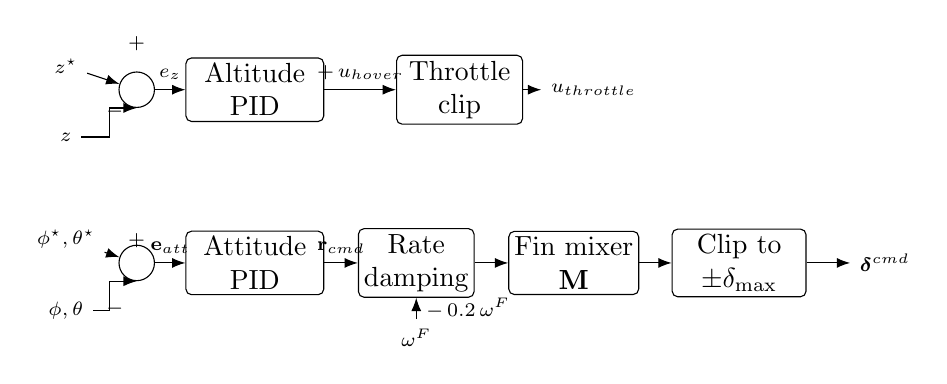
\begin{tikzpicture}[
    x=1cm,
    y=1cm,
    >={Latex[length=2.5mm]},
    block/.style={draw, rounded corners=2pt, align=center, minimum width=1.55cm, minimum height=0.78cm, inner sep=2pt},
    smallblock/.style={draw, rounded corners=2pt, align=center, minimum width=1.25cm, minimum height=0.78cm, inner sep=2pt},
    sum/.style={draw, circle, inner sep=0pt, minimum size=4.5mm},
    note/.style={align=center, font=\scriptsize},
    line/.style={-Latex, line width=0.4pt}
]
\node[note] (href) at (-0.2,2.0) {$z^\star$};
\node[note] (zmeas) at (-0.2,1.1) {$z$};
\node[sum] (sumz) at (0.7,1.7) {};
\node[block, minimum width=1.75cm] (pidz) at (2.2,1.7) {Altitude\\PID};
\node[block, minimum width=1.6cm] (throttle) at (4.8,1.7) {Throttle\\clip};
\node[note] (uthr) at (6.5,1.7) {$u_{throttle}$};

\node[note] (attref) at (-0.2,-0.2) {$\phi^\star,\theta^\star$};
\node[note] (attmeas) at (-0.2,-1.1) {$\phi,\theta$};
\node[sum] (sumatt) at (0.7,-0.5) {};
\node[block, minimum width=1.75cm] (pidatt) at (2.2,-0.5) {Attitude\\PID};
\node[smallblock] (damp) at (4.25,-0.5) {Rate\\damping};
\node[block, minimum width=1.55cm] (mixer) at (6.25,-0.5) {Fin mixer\\$\mathbf{M}$};
\node[block, minimum width=1.7cm] (clip) at (8.35,-0.5) {Clip to\\$\pm\delta_{\max}$};
\node[note] (delta) at (10.2,-0.5) {$\boldsymbol{\delta}^{cmd}$};
\node[note] (omegameas) at (4.25,-1.45) {$\omega^F$};

\draw[line] (href) -- (sumz);
\draw[line] (zmeas) -- ++(0.55,0) |- (sumz.south);
\draw[line] (sumz) -- node[above, font=\scriptsize] {$e_z$} (pidz);
\draw[line] (pidz) -- node[above, font=\scriptsize] {$+\,u_{hover}$} (throttle);
\draw[line] (throttle) -- (uthr);

\draw[line] (attref) -- (sumatt);
\draw[line] (attmeas) -- ++(0.55,0) |- (sumatt.south);
\draw[line] (sumatt) -- node[above, font=\scriptsize] {$\mathbf{e}_{att}$} (pidatt);
\draw[line] (pidatt) -- node[above, font=\scriptsize] {$\mathbf{r}_{cmd}$} (damp);
\draw[line] (damp) -- (mixer);
\draw[line] (mixer) -- (clip);
\draw[line] (clip) -- (delta);
\draw[line] (omegameas) -- node[right, font=\scriptsize] {$-\,0.2\,\omega^F$} (damp.south);

\node[note] at (0.7,2.28) {$+$};
\node[note] at (0.42,1.42) {$-$};
\node[note] at (0.7,-0.22) {$+$};
\node[note] at (0.42,-1.08) {$-$};
\end{tikzpicture}
}
\caption{Simplified PID controller signal flow. The altitude loop regulates vertical error and produces throttle after adding the hover bias $u_{hover}$. The attitude loop regulates roll and pitch, applies body-rate damping, and maps the resulting rate command to four fin commands through the mixer in (\ref{eq:fin_mixer}), ordered as front, right, rear, and left.}
\label{fig:pid_setup}
\end{figure}

\subsubsection{Shared RL Interface}

The current repo gives both RL variants the same control interface as PID:
\begin{itemize}
    \item \textbf{Observation}: the 24-dimensional vector in (\ref{eq:obs}).
    \item \textbf{Action}: four fin-angle targets and one throttle scalar, as in (\ref{eq:action_vector}).
    \item \textbf{Reward}: the same task-specific weighted sum in (\ref{eq:reward_sum}).
    \item \textbf{Task branches}: the same policy interface is evaluated on two task branches, hover and landing, using different reward weightings and spawn envelopes.
\end{itemize}

For the current code base, hover and landing are the two operative trajectory branches of the environment. The hover branch uses a 30 s horizon around a 5 m altitude target, while the landing branch uses a 60 s horizon with a ground-centered pad target and a wider spawn envelope. The benchmark campaign is therefore a controller comparison across the same physics and observation pipeline but different mission branches.

\subsubsection{PPO-MLP Baseline Design}

The present repository includes a PPO adapter and training entrypoint scaffold, but not yet a completed training loop. The project training specification defines the planned PPO baseline as a reactive actor-critic without temporal memory. In that design, the observation at a single step is processed by two separate multilayer perceptrons:
\begin{equation}
\pi_{\theta}: \mathbb{R}^{d_o}\rightarrow \mathbb{R}^{5}\times\mathbb{R}^{5},
\qquad
V_{\psi}: \mathbb{R}^{d_o}\rightarrow \mathbb{R},
\label{eq:ppo_actor_critic}
\end{equation}
where $d_o$ is the observation dimension. The training-plan specification uses a 20-dimensional observation for the future standalone training environment, while the current Isaac implementation uses 24 dimensions. In both cases, the architectural idea is the same: a feed-forward policy branch and a separate value branch.

The planned PPO-MLP architecture is:
\begin{itemize}
    \item policy branch: input $\rightarrow 256 \rightarrow 256 \rightarrow$ action mean and log-standard-deviation,
    \item value branch: input $\rightarrow 256 \rightarrow 256 \rightarrow 1$,
    \item hidden activation: \texttt{tanh},
    \item action distribution: Gaussian policy before adapter-based scaling.
\end{itemize}

In the current Isaac repo, the PPO adapter assumes the raw network output already lies in $[-1,1]$ and scales it to the physical action range:
\begin{equation}
\delta_i^{cmd} = \delta_{max}\,a_i^{raw},
\qquad
u_t = \frac{a_5^{raw}+1}{2}.
\label{eq:ppo_scaling}
\end{equation}
This makes the PPO baseline a purely reactive controller: it sees the current observation, produces one action, and does not explicitly preserve memory across steps.

Figure \ref{fig:ppo_architecture} summarizes the planned PPO-MLP baseline as a feed-forward actor-critic with separate policy and value branches.

\begin{figure*}[!t]
\centering
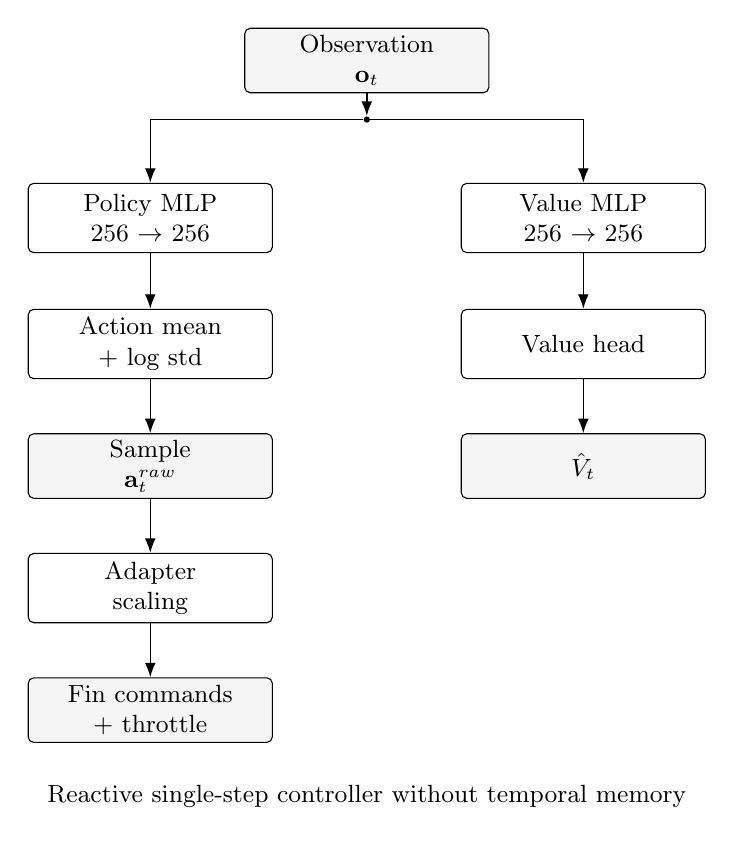
\begin{tikzpicture}[
    x=1cm,
    y=1cm,
    >={Latex[length=2mm]},
    box/.style={draw, rounded corners=2pt, align=center, minimum width=3.1cm, minimum height=0.88cm, inner sep=2pt, font=\small},
    io/.style={draw, rounded corners=2pt, align=center, minimum width=3.1cm, minimum height=0.82cm, inner sep=2pt, fill=gray!8, font=\small},
    dot/.style={circle, fill, inner sep=0.8pt},
    line/.style={-Latex, line width=0.5pt}
]
\node[io] (obs) at (0,0) {Observation\\$\mathbf{o}_t$};
\node[dot] (splitobs) at (0,-0.75) {};
\node[box] (actor) at (-2.75,-2.0) {Policy MLP\\256 $\rightarrow$ 256};
\node[box] (critic) at (2.75,-2.0) {Value MLP\\256 $\rightarrow$ 256};
\node[box] (policy) at (-2.75,-3.6) {Action mean\\+ log std};
\node[io] (raw) at (-2.75,-5.15) {Sample\\$\mathbf{a}^{raw}_t$};
\node[box] (scale) at (-2.75,-6.7) {Adapter\\scaling};
\node[io] (phys) at (-2.75,-8.25) {Fin commands\\+ throttle};
\node[box] (value) at (2.75,-3.6) {Value head};
\node[io] (vhat) at (2.75,-5.15) {$\hat{V}_t$};
\node[font=\small, align=center] at (0,-9.35) {Reactive single-step controller without temporal memory};

\draw[line] (obs.south) -- (splitobs);
\draw[line] (splitobs) -- ++(-2.75,0) -- (actor.north);
\draw[line] (splitobs) -- ++(2.75,0) -- (critic.north);
\draw[line] (actor) -- (policy);
\draw[line] (policy) -- (raw);
\draw[line] (raw) -- (scale);
\draw[line] (scale) -- (phys);
\draw[line] (critic) -- (value);
\draw[line] (value) -- (vhat);
\end{tikzpicture}
\caption{Planned PPO-MLP baseline. A single observation is processed by separate policy and value MLP branches; the sampled raw action is then mapped to four fin commands and one throttle command by the controller adapter.}
\label{fig:ppo_architecture}
\end{figure*}

\subsubsection{GTrXL-PPO Design}

The GTrXL-PPO controller extends PPO by replacing the purely reactive encoder with a temporal transformer backbone. As with PPO-MLP, the current repository implements the adapter and memory interface but not yet the full training loop. The training-plan design specifies a shared temporal encoder followed by separate policy and value heads:
\begin{equation}
\mathbf{h}_t = f_{\mathrm{GTrXL}}(\mathbf{o}_{t-L+1:t}, \mathbf{m}_{t-1}),
\label{eq:gtrxl_hidden}
\end{equation}
\begin{equation}
\pi_{\theta}(\mathbf{h}_t)\rightarrow \mathbf{a}^{raw}_t,
\qquad
V_{\psi}(\mathbf{h}_t)\rightarrow \hat{V}_t,
\label{eq:gtrxl_heads}
\end{equation}
where $\mathbf{m}_{t-1}$ is segment memory carried across the episode. In the planned benchmark design:
\begin{itemize}
    \item the input observation is first projected to a model dimension of 128,
    \item the temporal encoder uses 2 GTrXL layers with 4 attention heads,
    \item segment length is 64 steps,
    \item memory length is 64 steps,
    \item feed-forward dimension is 512,
    \item policy and value heads each use a 256-unit hidden layer.
\end{itemize}

The gating idea follows Parisotto et al. \cite{parisotto2020}: each transformer block can interpolate between residual passthrough and attention-enhanced output. Conceptually,
\begin{equation}
\mathbf{z}_{out}
=
\sigma(\mathbf{g})\odot \mathrm{Attn}(\mathbf{z}_{in})
+
\left(1-\sigma(\mathbf{g})\right)\odot \mathbf{z}_{in},
\label{eq:gtrxl_gate}
\end{equation}
which improves RL stability by preventing the transformer from forcing aggressive temporal mixing early in training.

This design gives GTrXL-PPO two advantages over the feed-forward PPO baseline. First, it can preserve a trajectory-level latent state over multiple seconds of descent, rather than inferring everything from a single observation. Second, under domain-randomized training, the memory state becomes an implicit task-identifier for the current disturbance realization. In that sense, the GTrXL branch is not only more robust but also more adaptive, because it can infer wind bias, delayed thrust response, or evolving landing phase from the observation trajectory itself.

The current adapter implements this design contract as
\begin{equation}
(\mathbf{a}^{raw}_t,\mathbf{m}_t) = f(\mathbf{o}_t,\mathbf{m}_{t-1}),
\label{eq:gtrxl_adapter}
\end{equation}
followed by the same physical action scaling used for PPO in (\ref{eq:ppo_scaling}). Memory is reset on episode boundaries, matching the intended training protocol.

Figure \ref{fig:gtrxl_architecture} summarizes the planned GTrXL-PPO controller as an attention-based actor-critic with recurrent memory and a shared temporal encoder.

\begin{figure*}[!t]
\centering
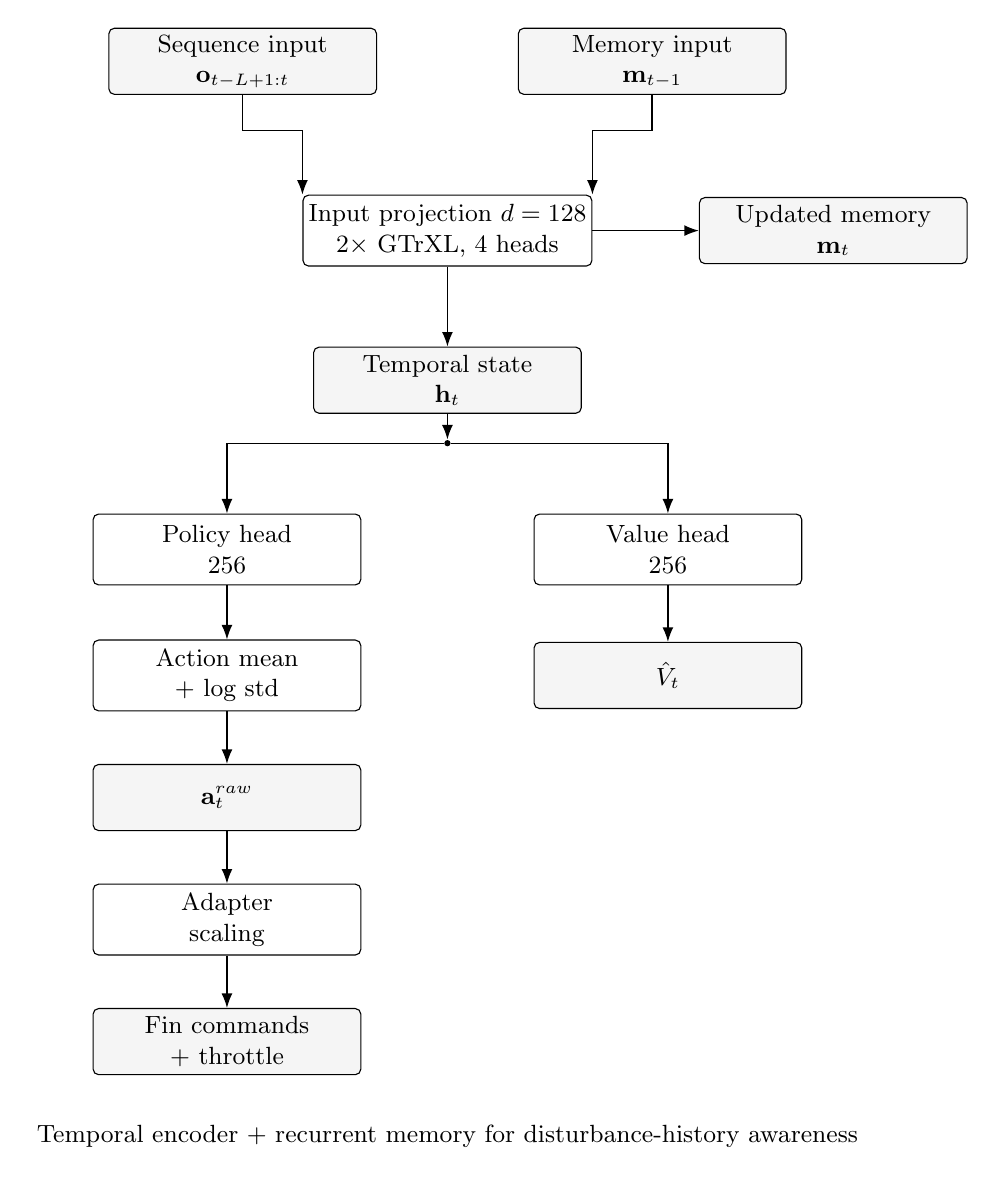
\begin{tikzpicture}[
    x=1cm,
    y=1cm,
    >={Latex[length=2mm]},
    box/.style={draw, rounded corners=2pt, align=center, minimum width=3.4cm, minimum height=0.9cm, inner sep=2pt, font=\small},
    io/.style={draw, rounded corners=2pt, align=center, minimum width=3.4cm, minimum height=0.84cm, inner sep=2pt, fill=gray!8, font=\small},
    dot/.style={circle, fill, inner sep=0.8pt},
    line/.style={-Latex, line width=0.5pt}
]
\node[io] (seq) at (-2.6,0) {Sequence input\\$\mathbf{o}_{t-L+1:t}$};
\node[io] (memin) at (2.6,0) {Memory input\\$\mathbf{m}_{t-1}$};
\node[box] (enc) at (0,-2.15) {Input projection $d=128$\\2$\times$ GTrXL, 4 heads};
\node[io] (latent) at (0,-4.05) {Temporal state\\$\mathbf{h}_t$};
\node[io] (memout) at (4.9,-2.15) {Updated memory\\$\mathbf{m}_t$};
\node[dot] (splitlatent) at (0,-4.85) {};
\node[box] (policyh) at (-2.8,-6.2) {Policy head\\256};
\node[box] (critic) at (2.8,-6.2) {Value head\\256};
\node[box] (policyout) at (-2.8,-7.8) {Action mean\\+ log std};
\node[io] (raw) at (-2.8,-9.35) {$\mathbf{a}^{raw}_t$};
\node[box] (scale2) at (-2.8,-10.9) {Adapter\\scaling};
\node[io] (phys2) at (-2.8,-12.45) {Fin commands\\+ throttle};
\node[io] (vhat2) at (2.8,-7.8) {$\hat{V}_t$};
\node[font=\small, align=center] at (0,-13.65) {Temporal encoder + recurrent memory for disturbance-history awareness};

\draw[line] (seq.south) -- ++(0,-0.45) -| (enc.north west);
\draw[line] (memin.south) -- ++(0,-0.45) -| (enc.north east);
\draw[line] (enc) -- (latent);
\draw[line] (enc.east) -- (memout.west);
\draw[line] (latent.south) -- (splitlatent);
\draw[line] (splitlatent) -- ++(-2.8,0) -- (policyh.north);
\draw[line] (splitlatent) -- ++(2.8,0) -- (critic.north);
\draw[line] (policyh) -- (policyout);
\draw[line] (policyout) -- (raw);
\draw[line] (raw) -- (scale2);
\draw[line] (scale2) -- (phys2);
\draw[line] (critic) -- (vhat2);
\end{tikzpicture}
\caption{Planned GTrXL-PPO controller. A sequence encoder with recurrent memory builds a latent temporal state before the policy and value heads split, allowing the controller to condition on disturbance history and landing phase.}
\label{fig:gtrxl_architecture}
\end{figure*}

\subsubsection{Trajectory Branches and Task-Specific Use}

For the paper and the benchmark plan, ``trajectory branches'' are used in two related senses. The first is \emph{environmental}: hover and landing are two task branches with different initial-condition envelopes, reward emphasis, and success criteria. The second is \emph{architectural}: both PPO-MLP and GTrXL-PPO are actor-critic methods with separate policy and value branches, while GTrXL additionally introduces a temporal encoding branch that processes observation sequences before those heads split.

This distinction is important in the final evaluation. The policy/value branch split affects optimization stability, while the hover/landing task split determines what behavior is being optimized. The GTrXL temporal branch is expected to matter most on the landing branch and especially under wind disturbance, where delayed recovery and implicit phase estimation become more important than in steady hover.

For readability, the principal symbols used throughout the mathematical development are collected in a notation summary near the end of the paper. Standard linear-algebra conventions are used throughout: bold lowercase variables denote vectors, bold uppercase variables denote matrices, subscripts index time or actuator elements, and superscripts indicate coordinate frames.

\section{Current Repository Status}

\subsection{Environment Architecture}

The implemented environment lives under \texttt{simulation/isaac/} and centers on a shared \texttt{TVCDirectRLEnv} interface. The environment uses a 120 Hz physics step with a decimation factor of 4, yielding an effective RL control rate of approximately 30 Hz. Each action contains four fin-angle commands and one throttle command. The observation vector contains 24 values: position error, quaternion attitude, body-frame linear velocity, body-frame angular velocity, altitude, four fin angles, four fin rates, normalized motor speed, and contact state.

The current physics stack includes:
\begin{itemize}
    \item EDF spool dynamics with first-order motor lag, thrust computation, rotor reaction torque, and gyroscopic terms.
    \item Servo dynamics with rate limiting and first-order lag.
    \item Semi-empirical fin aerodynamics with per-fin force computation and geometric center-of-pressure dispatch.
    \item Wind disturbance and body drag in the implemented disturbance path.
    \item Contact state management, crash logic, and randomized episode resets for hover and landing tasks.
\end{itemize}

Two tasks are already configured: hover at 5 m altitude and landing on a pad centered at the origin. The landing task includes touchdown softness, pad accuracy, and crash penalties in the reward structure. Hover emphasizes position error, tilt, drift, and no-contact stability.

\subsection{Controllers and Training State}

The repository contains three controller-side entry points relevant to this paper. First, a PID adapter maps altitude and attitude regulation into four fin angles plus throttle. Second, a PPO adapter provides action scaling for a future feed-forward PPO policy. Third, a GTrXL adapter manages the same action scaling while preserving transformer memory across episode steps. At present, only the adapter and script scaffolding are implemented for PPO and GTrXL-PPO; the actual training loop is still a stub awaiting integration with an external RL library.

This implementation detail matters for the paper. The project proposal includes broader comparison against SCP and full simulation-to-hardware transfer, but the current repository currently supports a near-term comparison centered on PID, PPO, and GTrXL-PPO. SCP remains part of the longer research plan, not the current code baseline.

\subsection{Implemented Versus Planned Disturbances}

The proposal discusses wind, sensor noise, center-of-mass shift, and fuel-slosh analogs. In the current repository state, the wind disturbance path is wired and tested. Configuration stubs also exist for center-of-mass shift and sensor noise, but those effects are not yet fully connected through the environment step loop. This paper therefore limits the near-term benchmark design to nominal conditions and wind-disturbed conditions, which are the two scenarios best supported by the code today.

\begin{table*}[!t]
\centering
\caption{Current repository implementation status at the time of writing.}
\label{tab:repo_status}
\scriptsize
\renewcommand{\arraystretch}{0.98}
\begin{tabularx}{\textwidth}{p{1.70in} p{1.05in} X}
\toprule
Component & Status & Evidence in repository \\
\midrule
6-DOF Isaac Sim environment & Implemented & \texttt{TVCDirectRLEnv} exposes reset/step/close, vectorized scene setup, task loading, reward assembly, and per-episode reset logic. \\
EDF propulsion and reaction torque & Implemented & EDF spool model, thrust model, and rotor reaction terms are coded with dedicated unit and simulation tests. \\
Servo, fin aero, and per-link force dispatch & Implemented & Servo dynamics, fin force model, center-of-pressure geometry, and wrench dispatch are present in the physics stack. \\
Wind disturbance path & Implemented & Wind drag and gust logic are wired through the environment and referenced by dedicated disturbance tests. \\
Contact and crash logic & Implemented & Contact state machine, crash criteria, touchdown cases, and landing termination logic are present. \\
Hover and landing tasks & Implemented & Separate task YAMLs define spawn envelopes, rewards, success criteria, and termination thresholds. \\
128-environment RL API & Implemented & Training configuration and smoke-test scaffolding exist for 128 parallel environments. \\
PID controller benchmark & Partially implemented & PID adapter and evaluation app exist, but no benchmark campaign has been reported yet in the repository. \\
PPO benchmark & Scaffold only & PPO adapter and training entrypoint exist, but the script still contains a stub loop and no trained policy. \\
GTrXL-PPO benchmark & Scaffold only & GTrXL adapter and training entrypoint exist, but no integrated transformer training loop has run yet. \\
Sensor-noise and CoM-shift disturbance study & Planned/partial & Config entries exist, but these disturbances are not yet fully wired into the runtime environment path. \\
HIL and hardware validation & Planned & Discussed in the proposal, but not implemented in the current repository. \\
\bottomrule
\end{tabularx}
\end{table*}

\section{Planned Benchmark Design}

\subsection{Evaluation Questions}

The benchmark design follows the research proposal while respecting current repository scope:
\begin{enumerate}
    \item Can the present Isaac Sim environment support stable hover and landing evaluation for an EDF thrust-vectoring proxy vehicle?
    \item How much improvement is expected from learned controllers over PID in nominal and wind-disturbed landing tasks?
    \item Does transformer memory plausibly provide an advantage over feed-forward PPO when the task includes delayed disturbance recovery and touchdown timing?
\end{enumerate}

\subsection{Near-Term Benchmark Protocol}

The near-term benchmark proposed for the repo consists of two simulation campaigns:
\begin{itemize}
    \item \textbf{Nominal campaign}: no injected disturbances, randomized spawn state within the configured task envelopes.
    \item \textbf{Wind campaign}: 2.0 m/s steady wind with 0.5 m/s lateral component, plus 5.0 m/s gusts lasting 0.5 s at randomized intervals, matching the current disturbance configuration.
\end{itemize}

For the work-in-progress study, a reasonable near-term benchmark would evaluate 100 hover episodes and 100 landing episodes per controller in the nominal campaign, then repeat 100 landing episodes in the wind campaign. The primary metrics are:
\begin{itemize}
    \item hover success rate,
    \item mean position error,
    \item maximum tilt,
    \item landing success rate,
    \item mean pad error,
    \item touchdown vertical speed,
    \item mean recovery time after a gust.
\end{itemize}

\subsection{Validation Evidence Already Available}

Although controller benchmarking is still pending, the code base is not empty. During preparation of this paper, the pure-Python unit-test suite in \texttt{simulation/isaac/tests/unit} was executed and all 82 tests passed. These tests cover math, geometry, quaternion handling, aerodynamic force logic, crash criteria, and rotor-reaction calculations. The repository also includes Isaac-dependent smoke tests for hover stability, vectorized 128-environment stepping, wind disturbance, touchdown transitions, and EDF spool response. Those Isaac-dependent tests support the intended benchmark path, even though the full controller campaign has not yet been run.

\section{Preliminary Validation Results}

\subsection{Actual Validation Status}

The strongest real result available today is code-level validation of the environment building blocks. The 82 passing unit tests indicate that the local math and dynamics components are internally consistent enough to justify moving into controller training. However, the project is still pre-benchmark. No trained PPO policy, no trained GTrXL-PPO policy, and no completed PID benchmark table exist yet in the repository. Table \ref{tab:actual_validation} summarizes the concrete validation evidence currently available.

\subsection{Projected Hover Benchmark}

Table \ref{tab:hover_projection} gives a preliminary projection for the hover task. These values are chosen to be consistent with the reward design, controller structure, and prior literature trend that learned policies improve precision while transformer memory improves temporal stability. They are not empirical results from this repository.

\begin{table*}[!t]
\centering
\begin{minipage}[t]{0.48\textwidth}
\centering
\captionof{table}{Actual validation evidence from the current repository.}
\label{tab:actual_validation}
\scriptsize
\setlength{\tabcolsep}{3pt}
\resizebox{\linewidth}{!}{%
\begin{tabular}{@{}lcc@{}}
\toprule
Validation item & Result & Type \\
\midrule
Pure-Python unit tests & 82/82 passed & Actual \\
Hover smoke-test specification & Present & Repo artifact \\
128-env RL API smoke test & Present & Repo artifact \\
Wind disturbance test & Present & Repo artifact \\
Touchdown state-machine test & Present & Repo artifact \\
EDF spool/reaction test & Present & Repo artifact \\
Controller benchmark tables & Not yet run & Actual status \\
\bottomrule
\end{tabular}
}
\end{minipage}\hfill
\begin{minipage}[t]{0.48\textwidth}
\centering
\captionof{table}{Projected hover performance under nominal conditions. Values are provisional estimates, not measured results.}
\label{tab:hover_projection}
\scriptsize
\setlength{\tabcolsep}{3pt}
\resizebox{\linewidth}{!}{%
\begin{tabular}{@{}lcccc@{}}
\toprule
Controller & Success (\%) & Mean err. (m) & Max tilt (deg) & Mean rate \\
\midrule
PID & 88 & 0.34 & 12.4 & 0.81 \\
PPO & 94 & 0.23 & 8.9 & 0.56 \\
GTrXL-PPO & 97 & 0.17 & 6.3 & 0.41 \\
\bottomrule
\end{tabular}
}
\end{minipage}
\end{table*}

The expected ordering is intuitive. PID can stabilize the vehicle near hover when the spawn envelope is modest, but it should remain the most sensitive to coupled lateral drift and attitude transients. PPO is expected to improve steady-state error through learned nonlinear control actions. GTrXL-PPO is projected to perform best because memory can help the policy interpret delayed actuator response and transient disturbance history over multiple control steps.

\subsection{Projected Landing Benchmark}

Table \ref{tab:landing_nominal_projection} shows projected nominal landing performance, and Table \ref{tab:landing_wind_projection} shows projected performance under the currently implemented wind-disturbance profile. These are provisional benchmark expectations that will be replaced by measured results once the controller campaign is complete.

\begin{table*}[!t]
\centering
\begin{minipage}[t]{0.48\textwidth}
\centering
\captionof{table}{Projected landing performance under nominal conditions. Values are provisional estimates, not measured results.}
\label{tab:landing_nominal_projection}
\scriptsize
\setlength{\tabcolsep}{3pt}
\resizebox{\linewidth}{!}{%
\begin{tabular}{@{}lccc@{}}
\toprule
Controller & Success (\%) & Pad error (m) & Touchdown vel. (m/s) \\
\midrule
PID & 86 & 0.27 & 0.61 \\
PPO & 92 & 0.18 & 0.46 \\
GTrXL-PPO & 96 & 0.11 & 0.35 \\
\bottomrule
\end{tabular}
}
\end{minipage}\hfill
\begin{minipage}[t]{0.48\textwidth}
\centering
\captionof{table}{Projected landing performance under wind disturbance. Values are provisional estimates, not measured results.}
\label{tab:landing_wind_projection}
\scriptsize
\setlength{\tabcolsep}{2pt}
\resizebox{\linewidth}{!}{%
\begin{tabular}{@{}lcccc@{}}
\toprule
Controller & Success (\%) & Pad error (m) & Touchdown vel. (m/s) & Recovery (s) \\
\midrule
PID & 71 & 0.38 & 0.75 & 1.9 \\
PPO & 83 & 0.24 & 0.57 & 1.2 \\
GTrXL-PPO & 89 & 0.16 & 0.42 & 0.8 \\
\bottomrule
\end{tabular}
}
\end{minipage}
\end{table*}

These projections show the qualitative story that the final benchmark is expected to test. First, all controllers degrade under wind, confirming that disturbance rejection should remain a central metric. Second, PPO is expected to outperform PID under both nominal and disturbed landings because the learned policy can better coordinate coupled throttle and fin commands. Third, GTrXL-PPO is projected to gain the largest advantage in the wind campaign, where temporal context matters most.

\section{Limitations and Next Steps}

The main limitation of this paper is deliberate: it is a work-in-progress manuscript written before the controller benchmark campaign has been completed. The projected numbers are not the result of executing PPO or GTrXL-PPO in the repository, and they must not be presented as experimental truth. They are provisional values intended to describe the planned comparative study while implementation is still underway.

The second limitation is implementation scope. The repository currently supports the environment, controller adapters, and wind disturbance path, but it does not yet include a full PPO training integration, a GTrXL training stack, an SCP baseline, or HIL/hardware execution. Likewise, the proposal's broader disturbance envelope, including center-of-mass shift and richer sensor-noise injection, remains future work in code even though the configuration hooks already exist.

The next steps are clear:
\begin{enumerate}
    \item integrate an RL training library for PPO and GTrXL-PPO;
    \item run nominal hover and landing benchmarks with reproducible seeds;
    \item run the wind campaign already supported by the present disturbance module;
    \item add missing disturbance pathways such as sensor noise and CoM variation;
    \item transition from simulation benchmarking to HIL and tethered hardware tests.
\end{enumerate}

\section{Conclusion}

This paper converts the current repository state into a work-in-progress research paper while staying honest about what has and has not been completed. The implemented project already contains a meaningful simulation artifact: a vectorized Isaac Sim environment for EDF thrust-vectoring control with actuator dynamics, aerodynamic force dispatch, wind disturbance, touchdown logic, and hover/landing task support. What it does not yet contain is the completed controller benchmark campaign promised in the research proposal.

For that reason, the value of this work-in-progress paper is twofold. First, it documents the real technical progress already achieved in the repository. Second, it provides clearly labeled projected benchmark tables that define the intended empirical comparison without overstating the current state of the research. If the next development phase successfully integrates PPO and GTrXL-PPO training, the projected tables in this manuscript can be replaced with empirical results and expanded into the full simulation-to-hardware validation study described in the original proposal.

\section{Notation Summary}
\label{sec:notation_summary}

Table \ref{tab:notation_kinematics} and Table \ref{tab:notation_control} summarize the principal symbols used in the mathematical development.

\begin{table*}[!t]
\centering
\caption{Kinematic, state, and frame notation used in the methodology section.}
\label{tab:notation_kinematics}
\scriptsize
\renewcommand{\arraystretch}{0.97}
\begin{tabularx}{\textwidth}{@{}p{1.25in}p{1.50in}X@{}}
\toprule
Symbol & Units / Type & Definition \\
\midrule
$\mathbf{R}_{I\leftarrow F}$ & $3\times 3$ matrix & Constant rotation that maps vectors from body-FRD coordinates to Isaac-aligned body coordinates. \\
$\mathbf{R}(\mathbf{q})$ & $3\times 3$ matrix & Rotation matrix associated with quaternion $\mathbf{q}$. \\
$\mathbf{q}=[w,x,y,z]^T$ & quaternion & Vehicle orientation stored in Isaac Lab convention. \\
$\mathbf{p}^{W}$ & m & Vehicle position in the Isaac world frame. \\
$\mathbf{v}^{W}$ & m/s & Vehicle linear velocity in the Isaac world frame. \\
$\mathbf{v}^{F}$ & m/s & Vehicle linear velocity expressed in body-FRD coordinates. \\
$\boldsymbol{\omega}^{W}$ & rad/s & Vehicle angular velocity in the world frame. \\
$\boldsymbol{\omega}^{F}$ & rad/s & Vehicle angular velocity expressed in body-FRD coordinates. \\
$\mathbf{x}_{t}$ & state vector & Full simulated state at time step $t$, including pose, velocity, fin state, rotor speed, and contact state. \\
$\mathbf{a}_{t}$ & action vector & Control command at time step $t$, consisting of four fin-angle commands and one throttle command. \\
$\mathbf{o}_{t}$ & observation vector & Policy observation at time step $t$, containing position error, attitude, body-frame velocities, altitude, fin states, normalized rotor speed, and contact state. \\
$\mathbf{e}_{p}$ & m & Position error, defined as $\mathbf{p}^{*}-\mathbf{p}$. \\
$\mathbf{p}^{*}$ & m & Task target position; for hover this is the hover point, and for landing this is the pad center. \\
$h$ & m & Altitude above ground. \\
$c_t$ & discrete state & Contact-state variable indicating airborne, candidate contact, landed, or crashed status. \\
$\phi,\theta$ & rad & Roll and pitch angles recovered from the vehicle quaternion. \\
$d_t$ & Boolean / indicator & Episode termination flag at time step $t$. \\
$\Delta t$ & s & Physics integration step used in each Isaac Lab substep. \\
$d$ & steps & Decimation factor, i.e., the number of physics substeps executed per RL action. \\
\bottomrule
\end{tabularx}
\end{table*}

\begin{table*}[!t]
\centering
\caption{Control, propulsion, aerodynamic, and reward notation used in the methodology section.}
\label{tab:notation_control}
\scriptsize
\renewcommand{\arraystretch}{0.97}
\begin{tabularx}{\textwidth}{@{}p{1.25in}p{1.50in}X@{}}
\toprule
Symbol & Units / Type & Definition \\
\midrule
$\delta_i$ & rad & Actual deflection of fin $i$ after servo dynamics. \\
$\delta_i^{cmd}$ & rad & Commanded deflection of fin $i$ before servo dynamics are applied. \\
$\delta_{\max}$ & rad & Maximum allowable fin deflection magnitude. \\
$\dot{\delta}_{\max}$ & rad/s & Maximum servo angular rate used in actuator saturation. \\
$\delta_{db}$ & rad & Servo deadband threshold. \\
$u_t$ & normalized scalar & Throttle command at time step $t$, constrained to $[0,1]$. \\
$u_{hover}$ & normalized scalar & Hover-throttle bias used by the PID controller. \\
$\tau_s$ & s & Servo first-order lag time constant. \\
$\Omega$ & rad/s & Current rotor angular speed. \\
$\Omega_{target}$ & rad/s & Rotor angular-speed target implied by the throttle command. \\
$\Omega_{\max}$ & rad/s & Maximum rotor angular speed in the EDF model. \\
$\tau_m$ & s & EDF motor spool time constant. \\
$T$ & N & Thrust magnitude generated by the EDF model. \\
$k_T$ & N\,s$^2$/rad$^2$ & Thrust coefficient in the quadratic thrust law $T=k_T\Omega^2$. \\
$k_Q$ & N\,m\,s$^2$/rad$^2$ & Reaction-torque coefficient in the quadratic rotor-torque law. \\
$I_r$ & kg\,m$^2$ & Rotor inertia used in spool and gyroscopic torque calculations. \\
$\mathbf{s}^{F}$ & unit vector & Rotor spin/exhaust axis expressed in body-FRD coordinates. \\
$\boldsymbol{\tau}_{static}$ & N\,m & Static reaction torque opposing rotor spin. \\
$\boldsymbol{\tau}_{spool}$ & N\,m & Dynamic torque produced by rotor angular acceleration. \\
$\boldsymbol{\tau}_{gyro}$ & N\,m & Gyroscopic precession torque produced by cross-coupling between body rate and rotor angular momentum. \\
$\rho$ & kg/m$^3$ & Air density used in the aerodynamic and drag models. \\
$v_{exh}$ & m/s & Nominal EDF exhaust speed used in the jet-vane pressure approximation. \\
$\bar{q}_{j}$ & Pa & Effective jet dynamic pressure seen by the fins. \\
$S$ & m$^2$ & Area of one fin. \\
$\alpha$ & rad & Fin deflection angle used in the aerodynamic coefficient model. \\
$C_N(\alpha)$ & coefficient & Normal-force coefficient for the jet-vane model. \\
$C_D(\alpha)$ & coefficient & Tangential-force coefficient for the jet-vane model. \\
$\mathbf{h}_i$ & unit vector & Hinge axis of fin $i$ in body-FRD coordinates. \\
$\mathbf{r}_i^{F}$ & m & Center-of-pressure offset of fin $i$ in body-FRD coordinates. \\
$\mathbf{F}_{i}^{F}$ & N & Body-frame force generated by fin $i$. \\
$\mathbf{F}_{EDF}^{F}$ & N & Body-FRD EDF thrust contribution before frame conversion and dispatch. \\
$\mathbf{F}_{body}^{F}$ & N & Combined body-level force, equal to EDF thrust plus optional wind/body-drag force. \\
$\mathbf{v}^{W}_{wind}$ & m/s & Wind velocity in world coordinates. \\
$\mathbf{v}^{W}_{rel}$ & m/s & Relative airflow velocity in world coordinates, computed as vehicle velocity minus wind velocity. \\
$\mathbf{v}_{xy}^{F}$ & m/s & Horizontal components of the body-FRD velocity vector. \\
$v_z^{F}$ & m/s & Vertical component of the body-FRD velocity vector; positive values denote downward motion. \\
$C_{D,b}$ & coefficient & Body drag coefficient used in the wind-disturbance model. \\
$A_b$ & m$^2$ & Reference area used in the body drag model. \\
$\mathcal{C}$ & configuration object & Merged runtime configuration assembled from task, environment, disturbance, and override dictionaries. \\
$\mathcal{E}$ & environment stack & Initialized Isaac Lab runtime stack including scene, interfaces, models, and managers. \\
$\mathbf{u}_t$ & control vector & Clamped action held constant across the $d$ physics substeps of one RL step. \\
$\Phi(\cdot)$ & transition map & One decimated simulation substep including actuation, force dispatch, and scene update. \\
$f_{act}(\cdot)$ & actuator map & Combined servo and EDF state update used in the force/wrench substep pipeline. \\
$f_{fin}(\cdot)$ & force map & Fin-force pipeline that produces per-fin body-frame forces and center-of-pressure data. \\
$\mathcal{W}^{(j)}$ & wrench data & External force/wrench data written to Isaac/PhysX at substep $j$. \\
$e_\theta$ & rad & Tilt-error magnitude, defined as $\sqrt{\phi^2+\theta^2}$. \\
$e_\omega$ & rad/s & Angular-rate magnitude, defined as $\|\boldsymbol{\omega}^{F}\|_2$. \\
$\overline{|\boldsymbol{\delta}|}$ & rad & Mean absolute fin deflection across the four fins. \\
$\overline{|\dot{\boldsymbol{\delta}}|}$ & rad/s & Mean absolute fin-rate magnitude across the four fins. \\
$\mathbb{1}_{(\cdot)}$ & indicator & Binary event indicator used for hover-within-tolerance, contact, crash, and landed states. \\
$r_{stay}$ & reward block & Constant alive-bonus contribution in the grouped reward presentation. \\
$r_{track}$ & reward block & State-tracking contribution based on position, tilt, angular-rate, or drift errors. \\
$r_{act}$ & reward block & Actuator-regularization contribution based on fin magnitude and fin-rate effort. \\
$r_{task}$ & reward block & Hover-specific task contribution based on staying inside the hover envelope and avoiding contact. \\
$r_{term}$ & reward block & Landing terminal-outcome contribution based on crash, landed state, and pad accuracy. \\
$r_{shape}$ & reward block & Landing descent-shaping contribution based on touchdown softness and approach speed. \\
$s_{soft}$ & scalar reward term & Touchdown-softness shaping term, defined as $\exp(-\max(v_z^{F},0))$. \\
$a_{pad}$ & scalar reward term & Pad-accuracy shaping term, defined as $\exp(-2\|\mathbf{p}_{xy}-\mathbf{p}^{*}_{xy}\|_2)$. \\
$K_{p,z},K_{i,z},K_{d,z}$ & controller gains & PID gains for the altitude loop. \\
$K_{p,a},K_{i,a},K_{d,a}$ & controller gains & PID gains for the attitude loop. \\
$\mathbf{M}$ & $4\times 3$ matrix & Fin-mixing matrix that maps roll, pitch, and yaw commands to four fin commands. \\
$\mathbf{m}_{t}$ & memory tensor & Transformer memory state carried across time in the GTrXL controller. \\
$L$ & steps & Sequence length used by the temporal encoder. \\
$\pi_{\theta}$ & policy mapping & Actor network parameterized by $\theta$. \\
$V_{\psi}$ & value mapping & Critic network parameterized by $\psi$. \\
$w_k$ & scalar weight & Weight applied to reward component $\phi_k(\mathbf{x}_t)$. \\
$\phi_k(\mathbf{x}_t)$ & reward term & The $k$th reward component evaluated from the current state. \\
\bottomrule
\end{tabularx}
\end{table*}

\section{Acknowledgment}

This manuscript was prepared from the current project repository, the research proposal, and the formatting/style of the prior conference paper example provided by the author. Projected benchmark values in this paper are provisional and are intentionally labeled as such pending empirical controller evaluation.

\begin{thebibliography}{99}

\bibitem{ackmese2007}
Ackmese, B., \& Ploen, S. R. (2007).
Convex programming approach to powered descent guidance for Mars landing.
\textit{Journal of Guidance, Control, and Dynamics}, 30(5), 1353--1366.

\bibitem{bushnell2018}
Bushnell, D. M., \& Moses, R. W. (2018).
Commercial space in the age of ``New Space,'' reusable rockets and the ongoing tech revolutions (NASA/TM-2018-220118).
NASA Langley Research Center.

\bibitem{carradori2025}
Carradori, J., Sagliano, M., \& Mooij, E. (2025).
Transformer-based robust feedback guidance for atmospheric powered landing.
In \textit{AIAA SciTech 2025 Forum} (AIAA Paper 2025-2771).
American Institute of Aeronautics and Astronautics.

\bibitem{dai2019}
Dai, Z., Yang, Z., Yang, Y., Carbonell, J., Le, Q. V., \& Salakhutdinov, R. (2019).
Transformer-XL: Attentive language models beyond a fixed-length context.
In \textit{Proceedings of the 57th Annual Meeting of the Association for Computational Linguistics} (pp. 2978--2988).

\bibitem{federici2024}
Federici, L., Zavoli, A., \& Furfaro, R. (2024).
Meta-reinforcement learning with transformer for lunar landing.
In \textit{AIAA SciTech 2024 Forum} (AIAA Paper 2024-2061).
American Institute of Aeronautics and Astronautics.

\bibitem{hwangbo2017}
Hwangbo, J., Sa, I., Siegwart, R., \& Hutter, M. (2017).
Control of a quadrotor with reinforcement learning.
\textit{IEEE Robotics and Automation Letters}, 2(4), 2096--2103.

\bibitem{konstantopoulos2020}
Konstantopoulos, G. C., Zheng, C., Papageorgiou, P. C., Tsourakis, G., Vournas, C. D., \& Alexandridis, A. T. (2020).
State-limiting PID controller for a class of nonlinear systems with constant uncertainties.
\textit{International Journal of Robust and Nonlinear Control}, 30(5), 1770--1787.

\bibitem{li2023}
Li, W., Luo, H., Lin, Z., Zhang, C., Lu, Z., \& Ye, D. (2023).
A survey on transformers in reinforcement learning.
\textit{Transactions on Machine Learning Research}.

\bibitem{parisotto2020}
Parisotto, E., Rae, J., Pascanu, R., Vinyals, O., et al. (2020).
Stabilizing transformers for reinforcement learning.
In \textit{Proceedings of the 37th International Conference on Machine Learning}.

\bibitem{schulman2017}
Schulman, J., Wolski, F., Dhariwal, P., Radford, A., \& Klimov, O. (2017).
Proximal policy optimization algorithms.
\textit{arXiv preprint arXiv:1707.06347}.

\end{thebibliography}

\end{document}
